% !TeX root = index.tex
\iffalse
This chapter presents the background physical or electrical theory
and on any analytical methods you will use to accomplish your goals.
If you have a research question, what is it?
Have you made any deductions from it that you are now testing?
What mathematical bases must be understood in order to interpret your results in Chapter 5?
Give the reader a solid understanding of the foundations here.
\fi

\iffalse
Figure \ref{fig:simple_blocks} represents simplified diagrams of RISC and OISC architectures. In RISC and CISC architecture, program data travels from program memory to the control block where instruction is decoded. Then control block further decides how data is directed in the datapath block which is described in section \ref{sec:datapath}. Such structure requires a complicated control block and additional data routing blocks. In order to increase performance of one such processor you would need to add pipelining or multiple cores. Both methods have disadvantages: multicore processor requires software adjustments and each core doubles the control and datapath blocks, substantially increasing transistor count; pipelinig allows operation at higher frequencies however it brings design complications such as complicated hazard prevention logic and instruction lookup. RISC architecture in this project is mainly based on theory in \autocite{harris_harris_2013}. The simplicity of OISC architecture overcomes these disadvantages:

Pipelining can be done by individual blocks and programmibly waiting for results, this is represented in figure \ref{fig:oisc_simple} Adder and Multiply vertical blocks, multicore can be simulated by adding more data and instruction buses, hazards can be prevented with software and/or integrated into address registers.
\\ 
ALU and other processor components can be divided by adding different address registers. This allow utilisation of multiple components at the same time given that multiple data buses are used. This is represented in figure \ref{fig:oisc_simple} Arithmetic Unit horizontal blocks. Assuming 4 data and instructions buses are used, \textbf{AND} and \textbf{OR} blocks sources A and B can all be written during one cycle utilising both blocks at the same time.
\\
These 
\\
\fi

In this section differences in RISC and OISC are explained. It includes predictions and theory behind it. 

This paper will be exploring is classical SISO processors. TTAs described section \ref{subsec:supporting_theory} are usually of type SIMT (single instruction, multiple transports) \autocite{289981}; A middle between these two classes is SIMO type (single instruction, multiple operation).

\subsection{RISC Processor}

\begin{figure*}[t!]
	\centering
	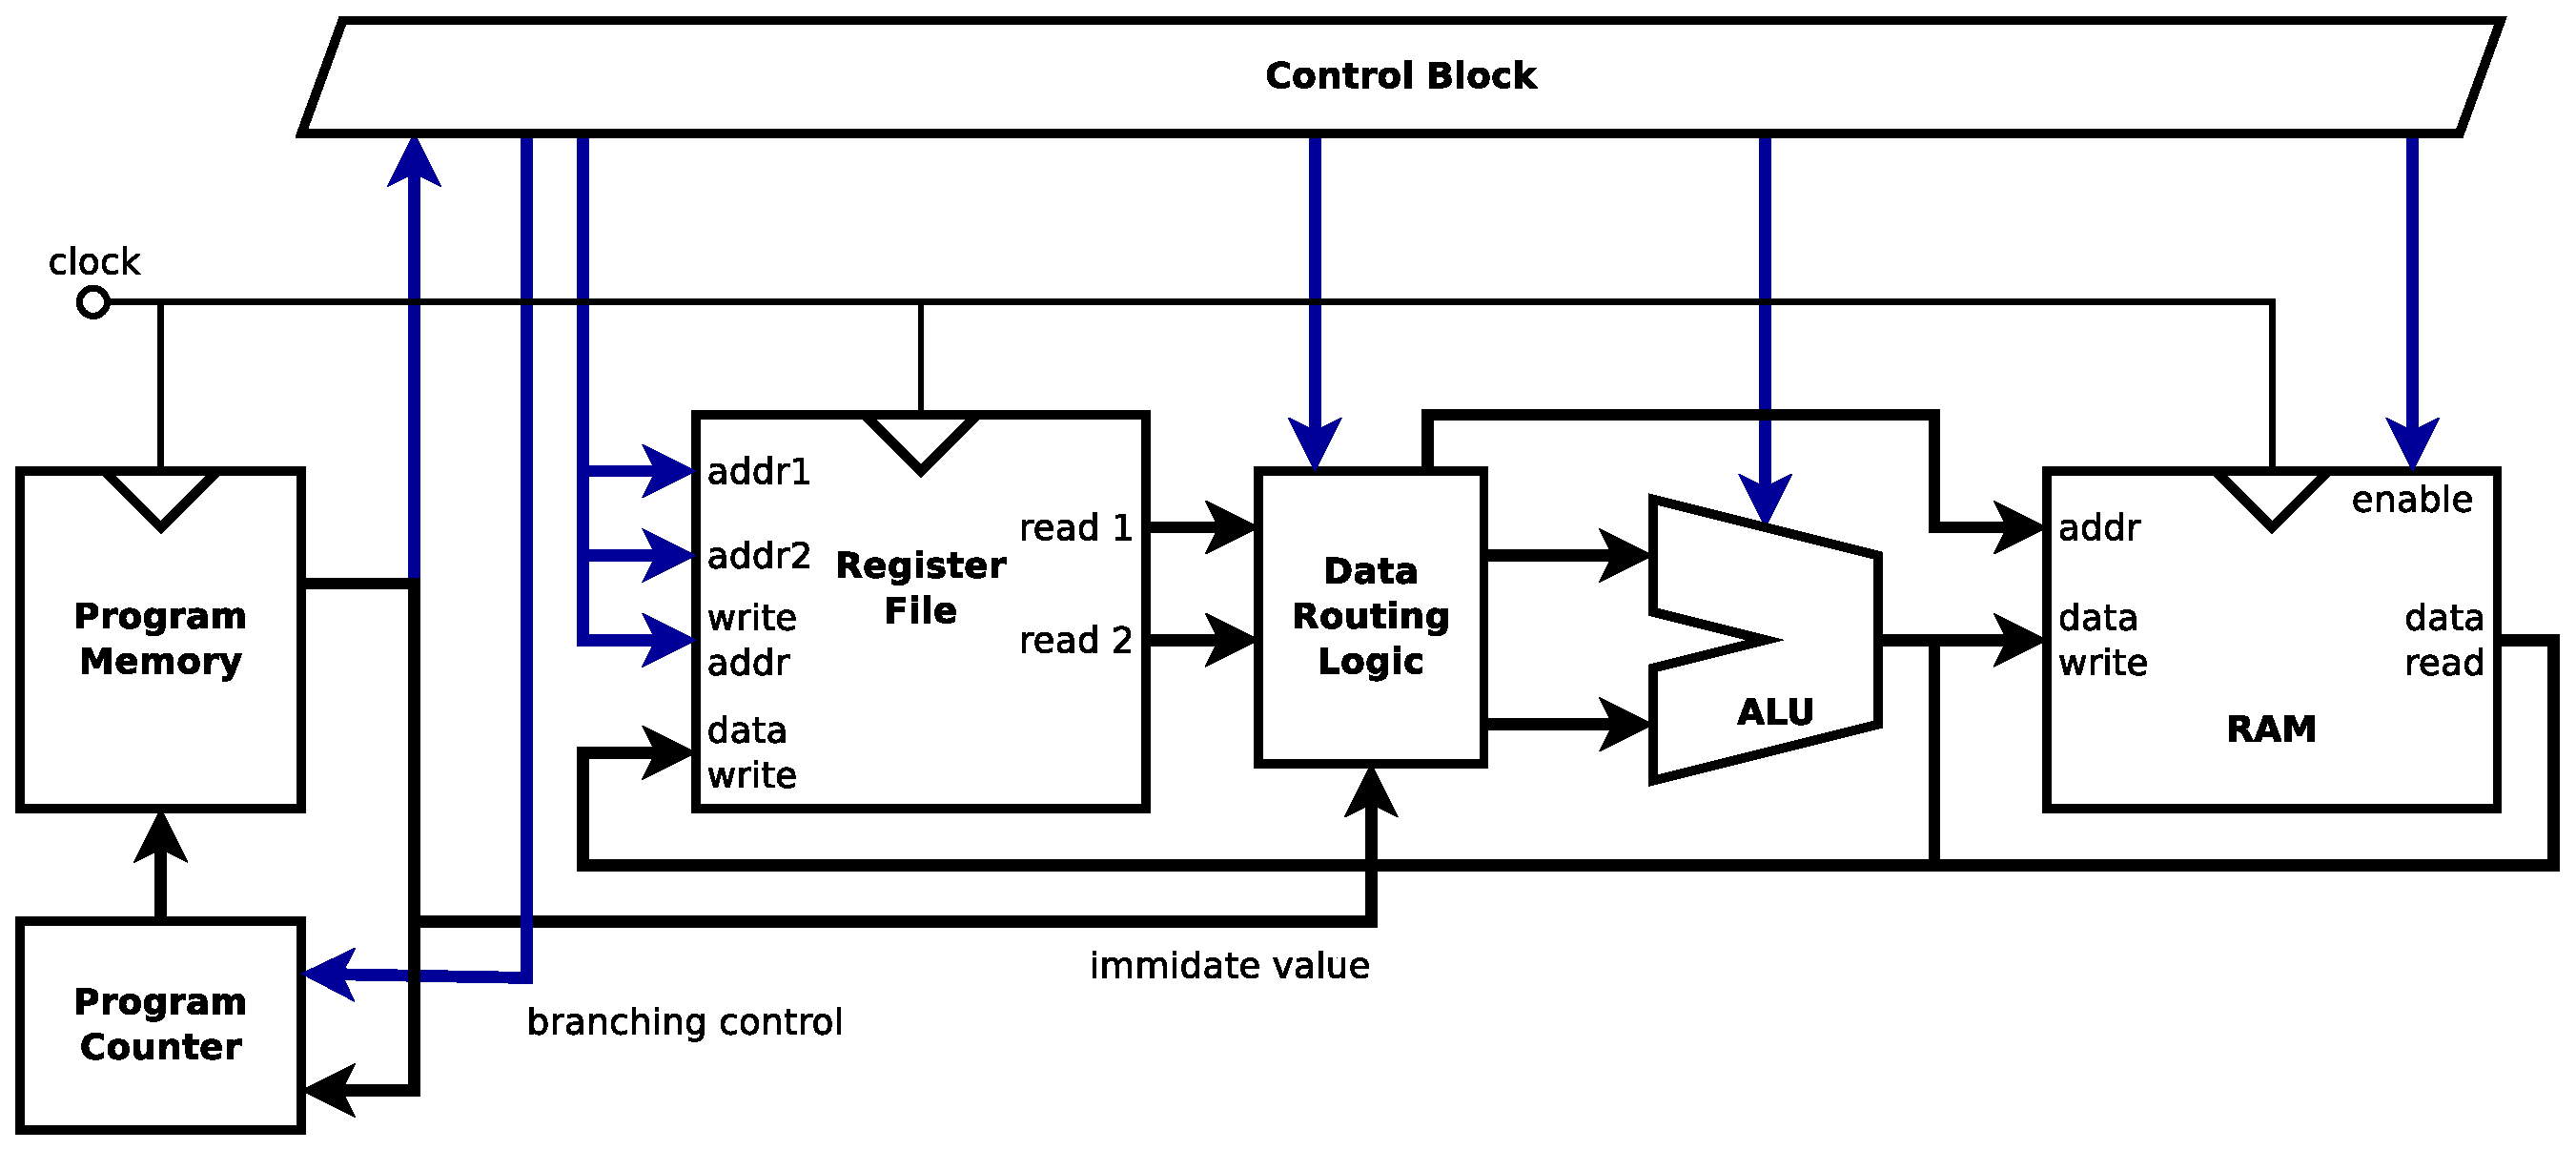
\includegraphics[width=\linewidth]{../resources/risc.eps}
	\caption{Abstract diagram of proposed RISC structure}
	\label{fig:risc_simple}
	
	\vspace{1cm}
	
	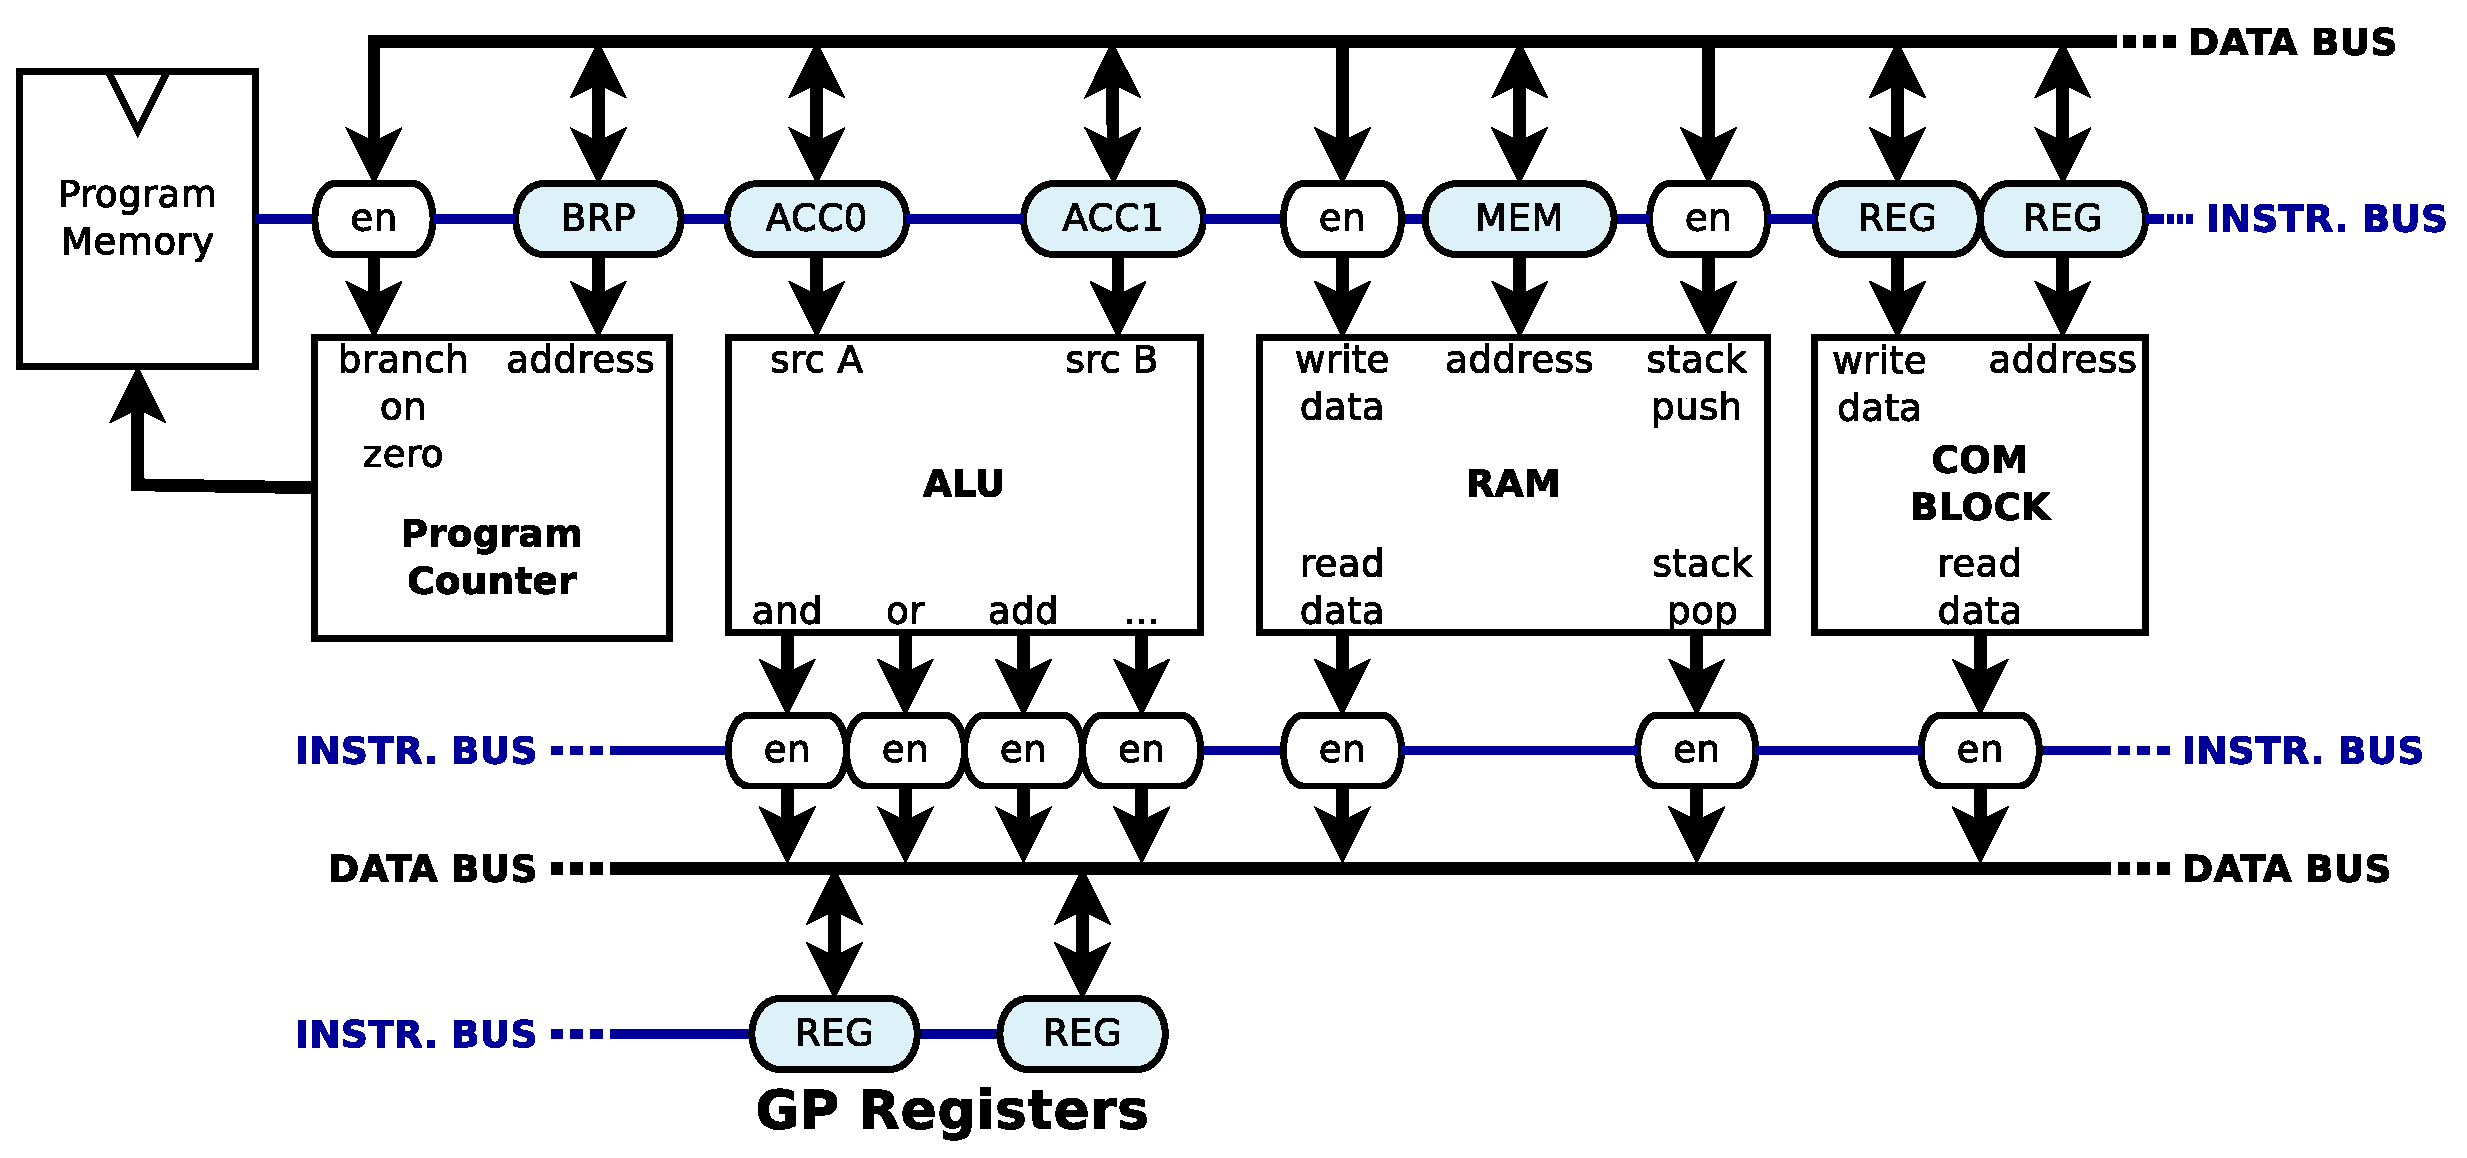
\includegraphics[width=\linewidth]{../resources/oisc.eps}
	\caption{Abstract diagram of proposed OISC structure}
	\label{fig:oisc_simple}
\end{figure*}

In this project, proposed RISC microarchitecture is mainly based on MIPS microachitecture \autocite{harris_harris_2013}. Figure \ref{fig:risc_simple} represents simplified diagram of proposed RISC processor. In this architecture, program data travels from program memory to the control block where instruction is decoded. Then control block further decides how data is directed in the datapath block. Such structure requires a complicated control block and additional data routing blocks. Depending on instruction, control block sets ALU, register file, memory operations and how data flows from one to other. Therefore, if non of blocks are bypassed, data can flow though every of these blocks, creating a log chain of combinational logic and increasing critical path. However this enables great flexibility allowing multiple operations to happen during single step, for example load value from register to memory, while address value is immediate offset by other register value using ALU. In order to increase performance of such processor, pipelining or multiple cores may be used.

\subsubsection{Pipelining}
\begin{multline}\label{eq:tc}
	\begin{split}
	T_c =& t_{pcq} + t_{ROM} + t_{register} + \\
	 	 & t_{routing} + t_{ALU} + t_{RAM} + t_{setup}
	\end{split}
\end{multline}

Equation \ref{eq:tc} shows maximum processor cycle period $T_c$ which depends on combinational logic delay of every logic block, flip-flop time of propagation from clock to output of synchronous sequential circuit $t_{pcq}$ and flip-flop setup time $t_{setup}$.

\begin{align}\label{eq:tcp}
	T_{cp} &= max \left( \begin{matrix}
	t_{pcq} + t_{ROM} + t_{setup},\\
	t_{pcq} + t_{register} + t_{setup},\\
	t_{pcq} + t_{ALU} + t_{setup},\\
	t_{pcq} + t_{RAM} + t_{setup}\\
	\end{matrix}\right)
\end{align}

Pipelinig separates each processor datapath block with a flip-flop. This changes combinational logic critical path this reducing cycle period. Pipelined processor cycle period $T_{cp}$ is represented in equation \ref{eq:tcp}. Such modification could technically increase clock frequency by 2 or 3 times.

Pipelining, however, introduces other design complications. Instructions that depend on each other, for example operation $R = A + B + C$ needs to be executed in two steps, $t = A + B$ and $R = t + C$. Second step is depends and previous step result. Therefore additional logic is required to detect such dependencies and bypass datapath stages, or stall pipelining. Furthermore, breaching would also require stalling, temporary saving datapath stage and restoring it if needed when branching is concluded, or further branch prediction logic. Such dependency and branching issue requires hazards prevention logic which increases processor complexity and required resources. 

\subsubsection{Multiple cores}

Multicore system is a solution to increase processor throughput by having multiple datapath and control logic instances, each running separate instructions. Cores share other resources such as RAM.

Multicore processor requires software adjustments as each processor core would execute separate programs. Therefore, some synchronisation between them is needed. A single additional core would also double the control and datapath blocks, substantially increasing resource requirements too. In addition, problems most often cannot be perfectly divided to parallel tasks due to some result dependencies between each task. Therefore, doubling processor core count would not likely result double the performance. 

\subsection{OISC Processor}

Figure \ref{fig:oisc_simple} represents simplified structure of OISC MOVE architecture. In simplest case, processor has a pair of buses - data and instruction. Instruction bus has source and destination address that connects two parts of processor via data bus. This mechanism allows data to flow around processor. Computation is accomplished by setting accumulators at destination addresses and taking computed values from source addresses. Other actions can be performed by at destination node for instance check value for branching or sending data to memory. 

\colorbox{yellow}{Needs to be finished.}

\subsection{Predictions}
\colorbox{yellow}{To be added.}
% Compare pipelining + software
\vfill




%There are many papers looking into application specific TTAs. 